\documentclass[a4paper, 10pt]{article}
\usepackage[p,osf]{scholax}
\usepackage{amsmath,amsthm}
\usepackage[scaled=1.075,ncf,vvarbb]{newtxmath}
\usepackage{graphicx}
\usepackage{mathtools}
\usepackage{tikz}
\usetikzlibrary {graphs,graphdrawing}
\usegdlibrary {trees}
\usetikzlibrary{calc, hobby}
\usepackage{float}
\author{So Okawara}
\date{\today}
\title{The Study of Game Theory on Graph}
\begin{document}
\maketitle
\section{Introduction}
Given each vertex $v_i$ on the graph $X$ has its \emph{benefit} $p_i(v_i)$, an \emph{input} $a \in v_i$ could convey \emph{signal} $x_a$ to $v_j$ by distribution of strategies $ p_n \in v_n$.\\\\
I.g., it could be optimised by DL for the given set of inputs $a_n \in A$ and its entries $v \in V$, to know the tendency in $A$ or $V$; like the network of financial system for the outer stimuli like the official discount rate. The second example is for \emph{topography} model of psychology by Freud, in more minute vertices, to model the unconsciousness. The third example is \emph{ecosystem} in general against any change outside.\\\\
In metaphor, if the pinball has \emph{Freud's pleasure principle} for the gross benefit $p^*$ as the score board on it, with the players as the environment to fit in, by learning the distribution of the springs dynamically; the pinball could have say it owns the mind to grow against the coming players, by \emph{conflict} among the springs set aside.\\\\
By this topography, i.g., conflict like ambivalent interpretation becomes possible like the image of a woman ``beautiful'' on topos $v_1$ while ``dangerous'' on topos $v_2$ with deciding how to output in the gross benefit $p^*$.
\section{On PyTorch}
As the easier case than AI, we firstly model the ideal financial market.
\begin{figure}[H]
\centering
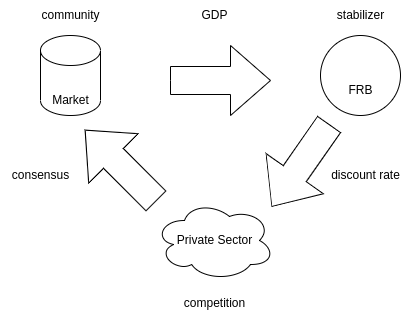
\includegraphics[width=10cm]
{trinity.png}
\caption{The ideal financial market}
\end{figure}
which could be a metaphor to the Freudian metanl model.
\begin{figure}[H]
\centering
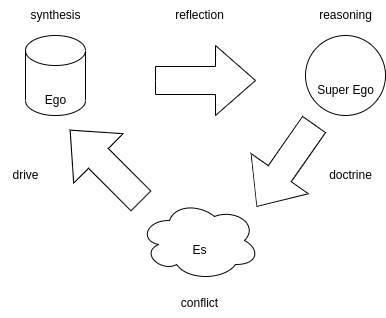
\includegraphics[width=10cm]
{topography.png}
\caption{The Freudian Topography}
\end{figure}
The weight matrix $W$ be on the cloud of private competitors; 
\begin{figure}[H]
\centering
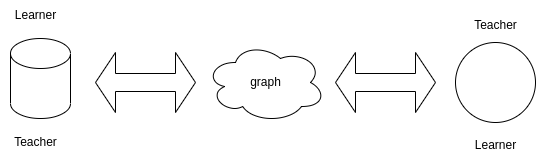
\includegraphics[width=12cm]
{pingpong.png}
\caption{Ping-pong Model}
\end{figure}

\section{In Theory}
Path-dependency 
best response function
\[ B_i(a_{-i}) = \{a_i \in A_i: u_i(a_i, a_{-i}) \ge u_i(a_i\prime, a_{-i}), \forall a_i\prime \in A_i\}\]
Cournot's oligopoly Game
\[ \pi_i (q_1, \cdots, q_n) = q_iP(q_1 + \cdots + q_n) - C_i(q_i)\]
The War of Attrition

\begin{equation}
     u_i(t_1,t_2) =
    \begin{aligned}
        & -t_i \quad &if \quad t_i < t_j\\
        & \cfrac{1}{2}v_i - t_i \quad &if \quad t_i = t_j\\
        & v_i - t_j \quad &if \quad t_i > t_j
    \end{aligned}
\end{equation} 
Accident Game
\[ -a_i -\rho (a_1,a_2) L(a_1,a_2)\]
\[ -a_2 - (1 - \rho (a_1, a_2)L(a_1,a_2))\]
\begin{thebibliography}{10}
\bibitem{game} An Introduction to Game Theory, Martin J. Osborne, 2000. 
\end{thebibliography}
\end{document}